\documentclass[12pt,a4paper]{article}
% Packages for enhanced functionality
\usepackage[utf8]{inputenc}
\usepackage[T1]{fontenc}
\usepackage{graphicx} % For including images
\usepackage{geometry} % For page layout
\usepackage{hyperref} % For clickable links and references
\usepackage{fancyhdr} % For custom headers and footers
\usepackage{float} 
\usepackage{circuitikz}
\usepackage{caption}
\usepackage{graphicx}
\usepackage{subcaption}
\usepackage{hyperref}
\usepackage{siunitx}
\usepackage{tikz}
\usepackage{circuitikz}
\usepackage{amsmath}
\usepackage{tikz}
\usepackage{subcaption}
\usepackage{booktabs}
\newcommand{\vecb}[1]{\mathbf{#1}}
\newcommand{\brak}[1]{\ensuremath{\left(#1\right)}}
\newcommand{\cbrak}[1]{\ensuremath{\left\{#1\right\}}}
\newcommand{\abs}[1]{\left\vert#1\right\vert}
\newcommand{\norm}[1]{\left\lVert#1\right\rVert}
\providecommand{\sbrak}[1]{\ensuremath{{}\left[#1\right]}}
\providecommand{\lsbrak}[1]{\ensuremath{{}\left[#1\right.}}
\providecommand{\rsbrak}[1]{\ensuremath{{}\left.#1\right]}}
\providecommand{\brak}[1]{\ensuremath{\left(#1\right)}}
\providecommand{\lbrak}[1]{\ensuremath{\left(#1\right.}}
\providecommand{\rbrak}[1]{\ensuremath{\left.#1\right)}}
\providecommand{\cbrak}[1]{\ensuremath{\left\{#1\right\}}}
\providecommand{\lcbrak}[1]{\ensuremath{\left\{#1\right.}}
\providecommand{\rcbrak}[1]{\ensuremath{\left.#1\right\}}}
\hypersetup{
    colorlinks=true,  % Enable colored text links
    linkcolor=orange,    % Internal links (sections, table of contents, etc.)
    urlcolor=orange,     % External URLs
    citecolor=orange,    % Citations
    pdfborder={0 0 0} % Remove ugly default borders
}


\title{\textbf{Lab Report: Experiment 6}}
\author{EE24BTECH11003 : Akshara Sarma Chennubhatla\\EE24BTECH11005 : Arjun Pavanje}

\begin{document}
\maketitle
\begin{center}
	\textbf{Experiment:\\}Measuring the I-V characteristics\\of a diode and determining\\Is and n. Finding small signal dynamic\\resistance(rd). Analyzing the\\DTFT of Id and determining\\harmonic amplitudes.
\end{center}
\vspace{30pt}
\begin{figure}[h!]
	\centering
	
\includegraphics[width = 100pt]{logo.png}\\
\end{figure}
\begin{center}
	Bachelor of Technology\\
	\vspace{10pt}
	Department of Electrical Engineering\\
\end{center}
\newpage

\section{Aim}

Plot the input and output characteristics of CE, CB, and CC configiutartions of BJT by plotting the family of curves obtained.

\section{Theory}

\subsection{Preliminaries}
The BJT is a three-terminal device with currents $I_E$, $I_B$ and $I_C$ satisfying
\begin{equation}
  I_E = I_B + I_C.\label{eq:em_rel}
\end{equation}
A widely used model (valid for forward- and reverse-active operation) is the Ebers--Moll model. In the forward-active regime, the collector current can be approximated by the diode-like expression
\begin{equation}
  I_C \approx I_{S} \exp\left(\frac{V_{BE}}{V_T}\right)\qquad (\text{for }V_{BE}\geq 100\,\text{mV}),\label{eq:ic_exp}
\end{equation}
where $I_S$ is the transistor saturation current and $V_T=kT/q\approx 25.85\,$mV at room temperature ($300\,$K). More generally, when the transistor is biased in forward-active region with a finite collector-base reverse bias, the practical relation is
\begin{equation}
  I_C = \beta_F I_B\approx \beta I_B\label{eq:ic_beta_ib}
\end{equation}
where $\beta_F$ (or simply $\beta$) is the forward DC current gain. The emitter current follows from \eqref{eq:em_rel}. In small-signal linearized analysis, the transconductance is
\begin{equation}
  g_m = \frac{\partial I_C}{\partial V_{BE}} = \frac{I_C}{V_T}.\label{eq:gm}
\end{equation}

Two limiting operating regions are important:
\begin{itemize}
  \item \textbf{Active region:} Base-emitter forward biased, base-collector reverse biased. Collector current is approximately controlled by $V_{BE}$ (or $I_B$) and weakly depends on $V_{CE}$ (finite output resistance).
  \item \textbf{Saturation region:} Both junctions forward biased. The transistor cannot sustain normal current gain and $I_C$ falls below $\beta I_B$; the device behaves like two forward diodes and the collector voltage drops near the emitter voltage.
\end{itemize}

\subsection{Common-Emitter (CE) configuration}
\paragraph{Definitions:}
For CE, the \emph{input} variables are $V_{BE}$ (or $I_B$) and the \emph{output} variables are $I_C$ and $V_{CE}$. The standard plots are:
\begin{enumerate}
  \item \emph{Input characteristic:} $I_B$ vs $V_{BE}$ at several fixed values of $V_{CE}$.  
  \item \emph{Output characteristic:} $I_C$ vs $V_{CE}$ for several fixed values of $I_B$.
\end{enumerate}

\paragraph{Input characteristic (CE):}
Using the diode-like behavior of the base-emitter junction, the input curve is exponential:
\begin{equation}
  I_B \propto I_{S,B} \exp\left(\frac{V_{BE}}{V_T}\right),\qquad \text{(approx.)}\label{eq:ib_vbe}
\end{equation}
where $I_{S,B}$ is an effective saturation parameter for the base-emitter junction that depends on geometry and doping. Thus the plot of $I_B$ vs $V_{BE}$ is a steeply rising exponential (on linear axes) or nearly linear on a semilog plot.

\paragraph{Output characteristic (CE):}
In forward-active region, for a given $I_B$ the collector current is approximately constant with $V_{CE}$:
\begin{equation}
  I_C \approx \beta I_B \quad(\text{flat} \;\text{region}),\label{eq:ic_flat}
\end{equation}
but with a slight slope due to the Early effect (modulation of the effective base width by $V_{CE}$). A common empirical model for the Early effect is
\begin{equation}
  I_C(V_{CE}) \approx I_{C0}\left(1+\frac{V_{CE}}{V_A}\right)\label{eq:early}
\end{equation}
where $V_A$ is the Early voltage (often tens to hundreds of volts). Equation \eqref{eq:early} explains why output curves are not perfectly horizontal but have a small positive slope.

The typical regions seen on the CE output plot are:
\begin{itemize}
  \item \textbf{Cutoff:} When $V_{BE}$ is too small, both $I_B$ and $I_C$ are near zero.
  \item \textbf{Active:} $I_C$ nearly constant with $V_{CE}$ (supply-limited by $I_B$ and $\beta$), small slope due to Early effect.
  \item \textbf{Saturation:} For small $V_{CE}$ (below $V_{CE(sat)}\sim 0.1$--$0.3\,$V), $I_C$ collapses and curves bend downward; $I_C < \beta I_B$.
\end{itemize}


\subsection{Common-Base (CB) configuration}
\paragraph{Definitions:}
For CB, the base is common and usually grounded; the \emph{input} is the emitter (voltage $V_{EB}$ or current $I_E$) and the \emph{output} is the collector ($I_C$ vs $V_{CB}$). The CB configuration emphasizes current gain $\alpha = I_C/I_E$ rather than $\beta$.

\paragraph{Input characteristic (CB):}
The emitter-base junction behaves like a forward diode so the emitter current depends exponentially on $V_{EB}$:
\begin{equation}
  I_E \propto I_{S,E}\exp\left(\frac{V_{EB}}{V_T}\right)\label{eq:ie_veb}
\end{equation}
As in CE, at large currents series resistance and high-level injection produce deviations.

\paragraph{Output characteristic (CB):}
The CB output plot shows $I_C$ vs $V_{CB}$ for fixed $I_E$. In the active region $I_C$ is nearly constant with $V_{CB}$ (for sufficiently large reverse bias) and equal to $\alpha I_E$:
\begin{equation}
  I_C \approx \alpha I_E\,.
\end{equation}
The slope with respect to $V_{CB}$ is typically even smaller than in CE (since the collector current is directly controlled by emitter injection and the device exhibits a large intrinsic output resistance in this topology).


\subsection{Common-Collector (CC) configuration (Emitter-follower)}
\paragraph{Definitions:}
In CC the collector is common (usually tied to supply); the \emph{input} is the base (voltage $V_{B}$ or base current $I_B$) and the \emph{output} is the emitter (voltage $V_E$ or current $I_E$).

\paragraph{Input characteristic (CC):}
Because the base-emitter junction still behaves like a diode, the input current $I_B$ depends exponentially on $V_{BE}$ (or $V_B-V_E$). However, when plotting $V_E$ vs $I_B$ or $V_B$ vs $I_B$, the presence of feedback (emitter follows base minus V_{BE}) changes the apparent slope.

\paragraph{Output characteristic (CC):}
A typical plot is emitter voltage $V_E$ versus collector-emitter voltage or versus load conditions. For moderate load changes the emitter tracks the base minus the diode drop:
\begin{equation}
  V_E \approx V_B - V_{BE} \approx V_B - 0.7\,\text{V} \quad (\text{approx. for silicon}).\label{eq:emitter_follow}
\end{equation}
If the base is driven by a source, the emitter output moves nearly one-for-one with the base (unity voltage gain less the diode drop), which explains the name emitter-follower. In terms of currents,
\begin{equation}
  I_E = (\beta+1) I_B\quad\Rightarrow\quad I_E/I_B = \beta+1.\label{eq:ie_ib}
\end{equation}
Thus a plot of $I_E$ vs $I_B$ is approximately linear with slope $\beta+1$.



\subsection{BJT DC parameters}
Parameters involved in BJT calculations,
\begin{align}
\beta &= \frac{I_C}{I_B} \quad \text{(current gain)} \\
\alpha &= \frac{I_C}{I_E} \quad \text{(current transfer ratio)} \\
\end{align}

where \(V_T = \dfrac{k_B T}{q} = {0.025875}V\) at $T=300K$
\pagebreak

\section{Experimental Setup}


\subsection{Circuit}
BJT available in the lab was model BC547 (npn), and values of resistance $R$ used are $150\Omega$ everywhere.
\begin{enumerate}
    \item Common Emitter
    \begin{figure}[ht!]
\centering
\resizebox{0.4\textwidth}{!}{%
\begin{circuitikz}
\tikzstyle{every node}=[font=\normalsize]
\draw (6.5,12.5) to[Tnpn, transistors/scale=1.19] (6.5,15);
\draw (5.5,13.75) to[R,l={ \normalsize $R_B$}] (3.75,13.75);
\draw (6.5,15) to[R,l={ \normalsize $R_C$}] (8.75,15);
\draw (3.75,13.75) to[american voltage source,l={ \normalsize $V_{in}$}] (3.75,11.25);
\draw (8.75,15) to[american voltage source,l={ \normalsize $V_C$}] (8.75,11.25);
\draw (3.75,11.25) to[short] (8.75,11.25);
\draw (6.5,12.5) to[short] (6.5,11.25);
\draw (6.5,11.25) to (6.5,11) node[sground]{};
\end{circuitikz}
}

\end{figure}
    \item Common Base
    \begin{figure}[!ht]
\centering
\resizebox{0.4\textwidth}{!}{%
\begin{circuitikz}
\tikzstyle{every node}=[font=\normalsize]
\draw (6.5,12.5) to[Tnpn, transistors/scale=1.19] (6.5,15);
\draw (6.5,15) to[R,l={ \normalsize $R_C$}] (8.75,15);
\draw (6.5,11.25) to[american voltage source,l={ \normalsize $V_{in}$}] (6.5,10);
\draw (8.75,15) to[american voltage source,l={ \normalsize $V_{C}$}] (8.75,11.25);

\draw (5.5,13.75) to (5,13.75) node[sground]{};
\draw (6.5,12.5) to[R,l={ \normalsize $R_E$}] (6.5,11.25);
\draw (6.5,10) to[short] (6.5,9.5);
\draw (6.5,9.5) to[short] (8.75,9.5);
\draw (8.75,9.5) to[short] (8.75,11.25);
\draw (8.75,9.5) to (8.75,9.25) node[sground]{};
\end{circuitikz}
}%

\end{figure}
\pagebreak
    \item Common Collector
    \begin{figure}[ht!]
\centering
\resizebox{0.4\textwidth}{!}{%
\begin{circuitikz}
\tikzstyle{every node}=[font=\normalsize]
\draw (6.5,12.5) to[Tnpn, transistors/scale=1.19] (6.5,15);

\draw (5.5,13.75) to[R,l={ \normalsize $R_B$}] (3.75,13.75);
\draw (6.5,12.5) to[R,l={ \normalsize $R_E$}] (6.5,10.75);
\draw (6.5,10.75) to[american voltage source,l={ \normalsize $V_E$}] (6.5,8.75);
\draw (3.75,13.75) to[american voltage source,l={ \normalsize $V_{in}$}] (3.75,8.75);
\draw (3.75,8.75) to[short] (6.5,8.75);
\draw (6.5,15) to (7.75,15) node[sground]{};
\draw (6.5,8.75) to (6.5,8.5) node[sground]{};
\end{circuitikz}
}%

\end{figure}
\end{enumerate}
Circuit pictures,
\begin{figure}[H]
    \centering
    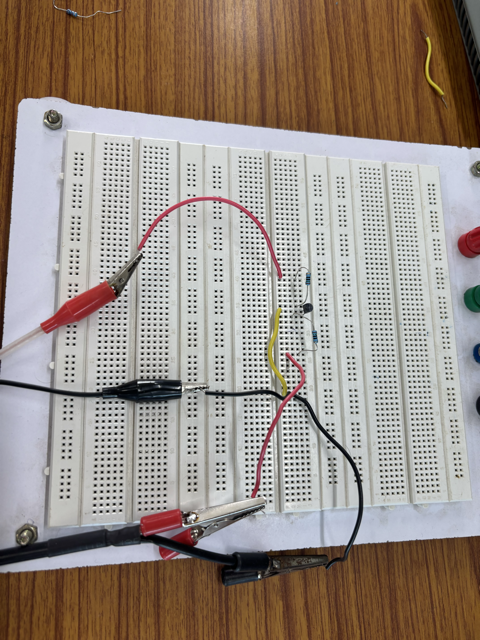
\includegraphics[angle = 90, width=0.8\textwidth]{Experiment_6/circuit_figs/circuit_1.png}
\end{figure}

\begin{figure}[H]
    \centering
    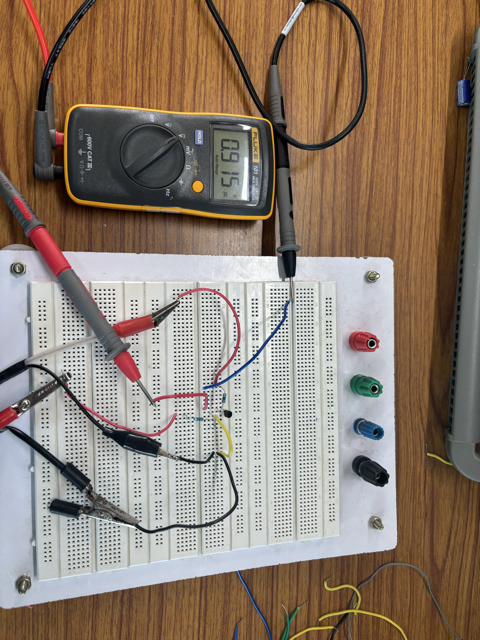
\includegraphics[angle = 90, width=0.8\textwidth]{Experiment_6/circuit_figs/circuit_2.png}
\end{figure}

\section{Procedure}

\subsection{Common Emitter Configuration}
\subsubsection{Output Characteristics}
\begin{enumerate}
    \item Connect the circuit as shown in the figure. 
    \item Keep $V_{BE}$ constant and vary $V_{CE}$ using a multimeter and taking appropriate step size.
    \item Repeat the above step for different values of $V_{BE}$ $(0.63, 0.65, 0.67)$ to obtain a family of curves.
    \item Since we can't directly measure current with a multimeter measure potential across the $R_C$ (since this is just a scaled version of $I_C$).
    \item Plot the family of $I_C$ vs $V_{CE}$ curves.
\end{enumerate}
\begin{figure}[H]
    \centering
    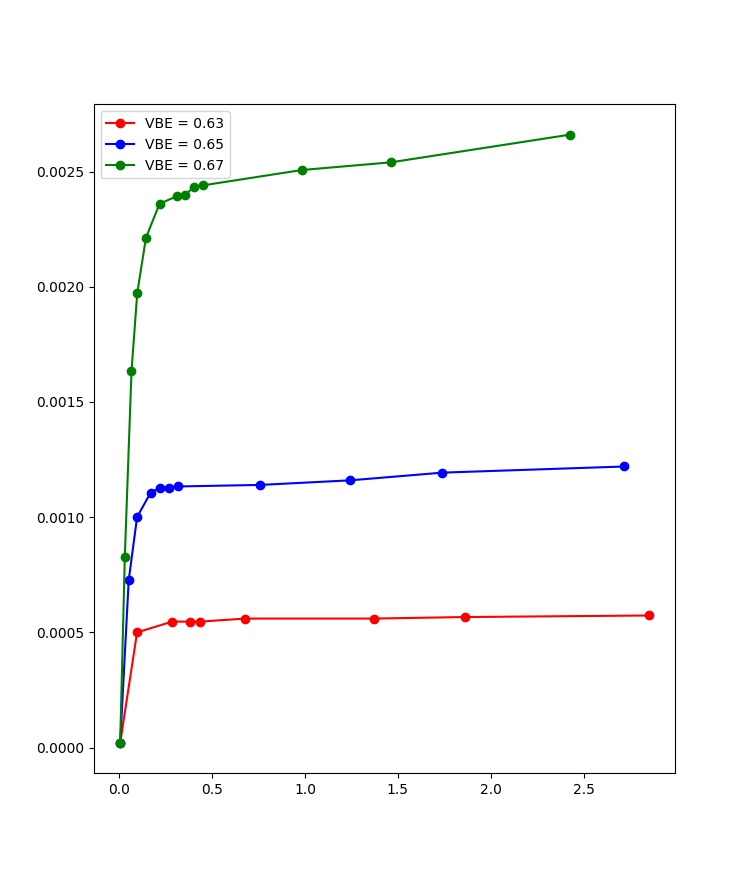
\includegraphics[width=0.8\textwidth]{Experiment_6/figs/ce_op.png}
\end{figure}

\subsubsection{Input Characteristics}
\begin{enumerate}
    \item Connect the circuit as shown in the figure. 
    \item Keep $V_{CE}$ constant and vary $V_{BE}$ using a multimeter and taking appropriate step size.
    \item Repeat the above step for different values of $V_{CE}$ $(0.2, 0.5, 0.6)$ to obtain a family of curves.
    \item Since we can't directly measure current with a multimeter measure potential across the $R_B$ (since this is just a scaled version of $I_B$).
    \item Plot the family of $I_B$ vs $V_{BE}$ curves.
\end{enumerate}
\begin{figure}[H]
    \centering
    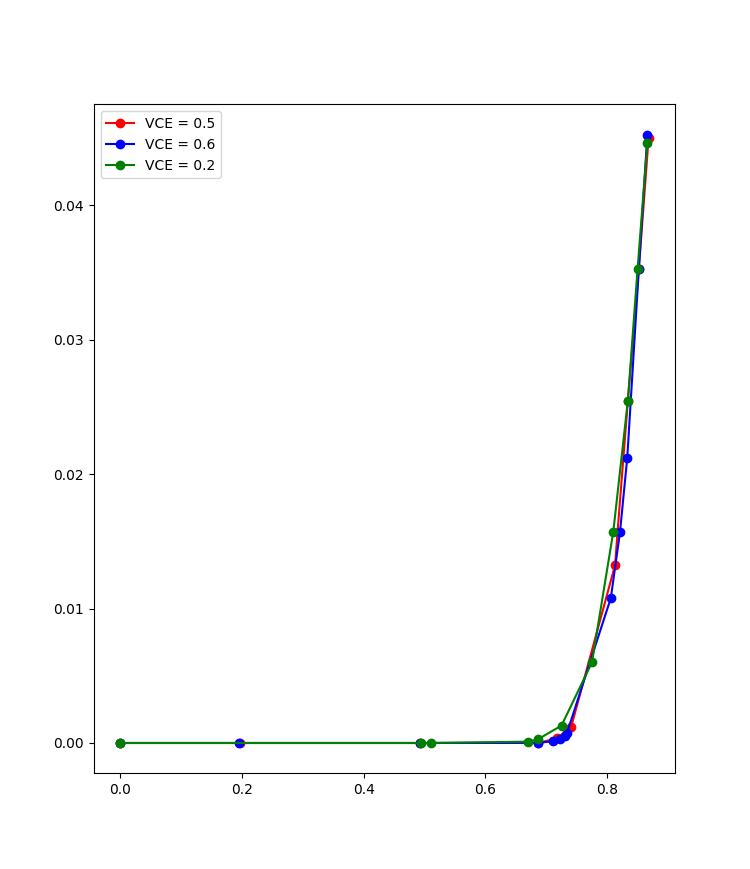
\includegraphics[width=0.8\textwidth]{Experiment_6/figs/ce_ip.png}
\end{figure}
\subsection{Common-Base Configuration}
\subsubsection{Output Characteristics}
\begin{enumerate}
    \item Connect the circuit as shown in the figure. 
    \item Keep $V_{BE}$ constant and vary $V_{CB}$ using a multimeter and taking appropriate step size.
    \item Repeat the above step for different values of $V_{BE}$ $(-2.5, -5, -7.5)$ to obtain a family of curves.
    \item Since we can't directly measure current with a multimeter measure potential across the $R_C$ (since this is just a scaled version of $I_C$).
    \item Plot the family of $I_C$ vs $V_{CB}$ curves.
\end{enumerate}
\begin{figure}[H]
    \centering
    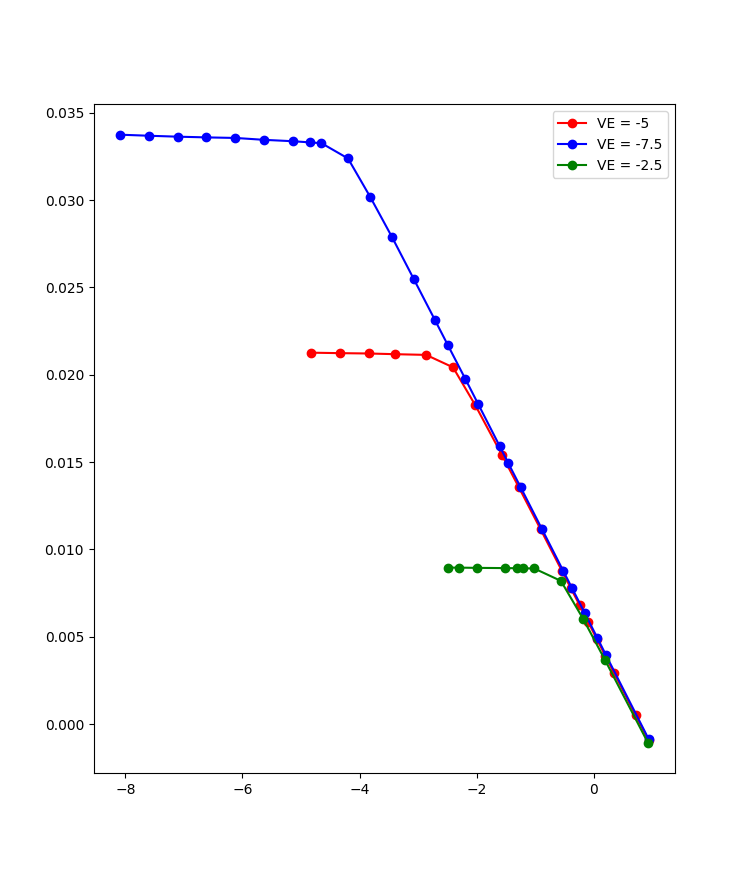
\includegraphics[width=0.8\textwidth]{Experiment_6/figs/cb_op.png}
\end{figure}
\subsubsection{Input Characteristics}
\begin{enumerate}
    \item Connect the circuit as shown in the figure. 
    \item Keep $V_{CB}$ constant and vary $V_{BE}$ using a multimeter and taking appropriate step size.
    \item Repeat the above step for different values of $V_{CB}$ $(-1,-2,-3)$ to obtain a family of curves.
    \item Since we can't directly measure current with a multimeter measure potential across the $R_E$ (since this is just a scaled version of $I_E$).
    \item Plot the family of $I_E$ vs $V_{BE}$ curves.
\end{enumerate}
\begin{figure}[H]
    \centering
    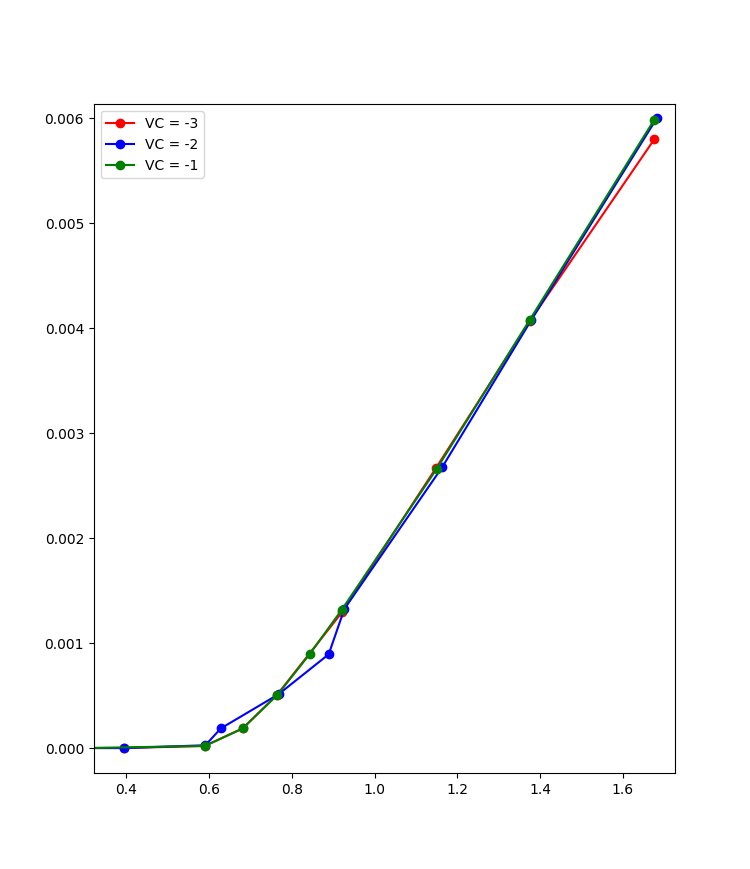
\includegraphics[width=0.8\textwidth]{Experiment_6/figs/cb_ip.png}
\end{figure}                

\subsection{Common-Collector Configuration}
\subsubsection{Output Characteristics}
\begin{enumerate}
    \item Connect the circuit as shown in the figure. 
    \item Keep $V_{CB}$ constant and vary $V_{CE}$ using a multimeter and taking appropriate step size.
    \item Repeat the above step for different values of $V_{CB}$ $(0.6, 0.65, 0.7)$ to obtain a family of curves.
    \item Since we can't directly measure current with a multimeter measure potential across the $R_E$ (since this is just a scaled version of $I_E$).
    \item Plot the family of $I_E$ vs $V_{CE}$ curves.
\end{enumerate}
\begin{figure}[H]
    \centering
    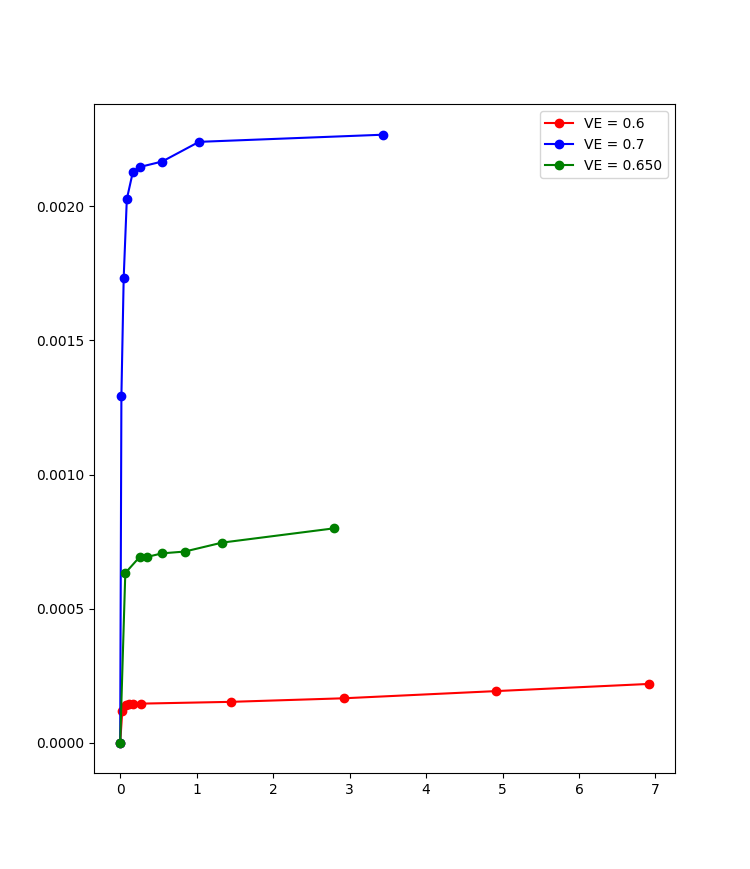
\includegraphics[width=0.8\textwidth]{Experiment_6/figs/cc_op.png}
\end{figure}
\subsubsection{Input Characteristics}
\begin{enumerate}
    \item Connect the circuit as shown in the figure. 
    \item Keep $V_{CE}$ constant and vary $V_{CB}$ using a multimeter and taking appropriate step size.
    \item Repeat the above step for different values of $V_{CE}$ $(0.6, 0.5, 1)$ to obtain a family of curves.
    \item Since we can't directly measure current with a multimeter measure potential across the $R_B$ (since this is just a scaled version of $I_B$).
    \item Plot the family of $I_B$ vs $V_{CB}$ curves.
\end{enumerate}
\begin{figure}[H]
    \centering
    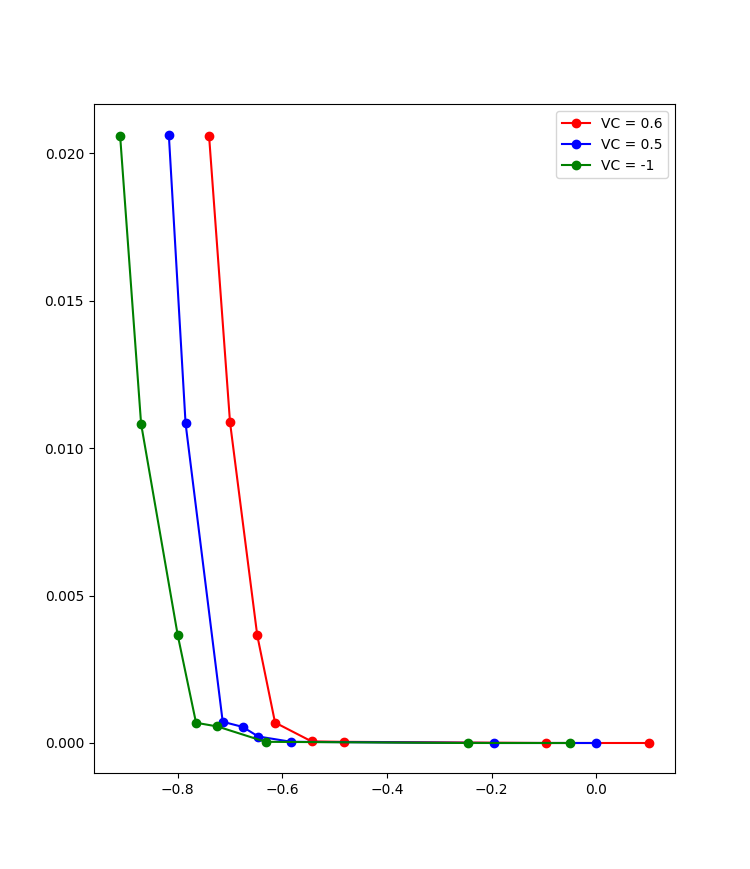
\includegraphics[width=0.8\textwidth]{Experiment_6/figs/cc_ip.png}
\end{figure}                


\section{Analysis}
\subsection{Input Characteristics}
All 3 configurations (CE, CB, CC) show exponential input characteristic, following Schottky's diode equation. This makes sense as an npn BJT is a diode which has 3 doped regions (n, p, followed by n). Hence we can expect a similar graph. 

\subsection{Output Characteristics}
All 3 configurations (CE, CB, CC) show similar graphs. The graphs have 3 regions,
\begin{itemize}
    \item Cutoff Region: Output current $\approx 0$
    \item Active Region: There is a linear relation between input and output.
    \item Saturation REgion: Output current goes into saturation i.e. remains constant.
\end{itemize}
Depending on configuration, output or input term varies but overall graph remains the same.

\section{Determination of DC current gain $\boldsymbol{\beta}$ in BJT configurations}

This section explains how to determine the DC current gain (commonly written $\beta$ or $h_{FE}$) of a bipolar junction transistor (BJT) in the three standard configurations: common-emitter (CE), common-base (CB) and common-collector (CC, emitter-follower). For each configuration we give the measurement procedure, the equations used to compute $\beta$ (or $\alpha$ where appropriate), and a worked numerical example using the CE value $\beta_{CE}=284.405046343$.  

\subsection{General definitions}
\begin{itemize}
  \item Collector current: $I_C$.
  \item Base current: $I_B$.
  \item Emitter current: $I_E$ (note $I_E=I_C+I_B$ exactly).
  \item DC current gain (common-emitter definition):
    \begin{equation}
      \beta_{DC} \equiv \beta = \frac{I_C}{I_B}.
    \end{equation}
  \item Forward current gain (common-base):
    \begin{equation}
      \alpha = \frac{I_C}{I_E}, \qquad \text{with}\quad \beta=\frac{\alpha}{1-\alpha},\quad \alpha=\frac{\beta}{\beta+1}.
    \end{equation}
\end{itemize}

\subsection{Common-Emitter (CE)}
\paragraph{Measurement procedure}
\begin{enumerate}
  \item Bias the transistor so it is in forward-active region.
  \item Hold $V_{CE}$ constant and sweep the base current $I_B$ across a suitable range (e.g. 10\,$\mu$A to 100\,$\mu$A in equal steps) using a current source or a series resistor and precise voltage reference.
  \item For each value of $I_B$ measure the resulting collector current $I_C$ and record the pair $(I_B,I_C)$.
\end{enumerate}

\paragraph{Data analysis}
If the transistor remains in the linear forward-active region, the relation
\begin{equation}
  I_C \approx \beta\,I_B
\end{equation}
holds. We can extract $\beta$ from experimental data by computing $\beta_i = I_{C,i}/I_{B,i}$ $\beta_i = I_{C,i}/I_{B,i}$ for each recorded point.

\paragraph{Worked numerical example}
Based on the different points recorded, the calculated value of $\beta$ comes out to be:
\begin{equation*}
  \beta_{CE} = 284.405046343,
\end{equation*}

\subsection{Common-Base (CB)}
\paragraph{Measurement procedure}
\begin{enumerate}
  \item Bias the collector-base junction in reverse (choose $V_{CB}$ such that the device is in the active region; typical experimental values: $V_{CB}=5$--$10\,$V).
  \item Sweep the emitter current $I_E$ (or vary emitter voltage while measuring $I_E$ and $I_C$). For each $I_E$ record $I_C$.
\end{enumerate}

\paragraph{Data analysis}
Compute the forward current gain
\begin{equation}
  \alpha = \frac{I_C}{I_E}.
\end{equation}
Convert $\alpha$ to $\beta$ when required via
\begin{equation}
  \beta = \frac{\alpha}{1-\alpha}.
\end{equation}

Thus, a CB measurement yielding $\alpha\approx 0.99650$ corresponds to $\beta\approx 284.405$ and this matches the value obtained in the other configuration. This matches the $\alpha$ value obtained by calculating $\dfrac{\alpha}{1-\alpha}$

\subsection{Common-Collector (CC)}
\paragraph{Measurement procedure}
\begin{enumerate}
  \item Keep the collector at a fixed voltage (connected to the supply so transistor is not saturating) and sweep $I_B$ (or the base voltage), measure the emitter current $I_E$ (and optionally $I_C$).
\end{enumerate}

\paragraph{Data analysis}
In the emitter-follower configuration the emitter current is related to the base current by
\begin{equation}
  I_E = (\beta+1)I_B.
\end{equation}
Hence one can compute
\begin{equation}
  \beta = \frac{I_E}{I_B} - 1.
\end{equation}

\section{Conclusion}

The experimental analysis successfully demonstrated the input and output characteristics of BJT in CE, CB, and CC configurations. Each configuration exhibits distinct properties making them suitable for specific applications. The CE configuration provides high gain, CB offers good high-frequency response, and CC serves as an effective buffer. The measured results closely match theoretical predictions, validating the understanding of BJT behavior in different configurations.

\end{document}